\begin{problem}{\#1 (20 points)}
    Using the bypass algorithm taught in class, convert each of the following TGs into regular expressions.
    \begin{enumerate}[label={\bf \alph*)}]
        \item 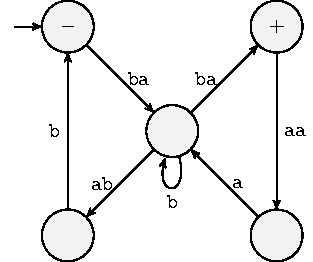
\includegraphics[]{figures/question/Question1A.pdf}
        \item 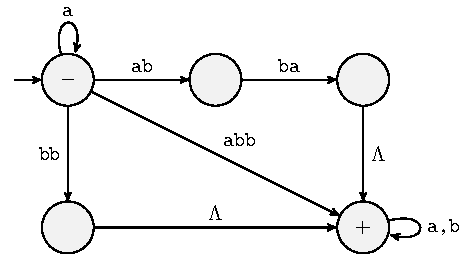
\includegraphics[]{figures/question/Question1B.pdf}
    \end{enumerate}
\end{problem}
\vspace{2em}
\begin{solution}
    \begin{enumerate}[label={\bf \alph*)}]
        \item \begin{enumerate}[label=\arabic*:]
            \item Start states should only have outgoing edges and end states should only have incoming edges.
            Move start and end states to fit this criteria.
            Label nodes that are not the start and end states.
            \newpage
            \begin{figure}[h!]
                \centering
                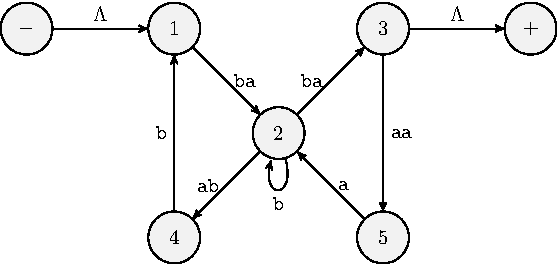
\includegraphics[]{figures/answer/Answer1A1.pdf}
                \caption*{Step 1: moving the start and end states.}
            \end{figure}
            \item Remove / bypass states 4 and 5.
            \begin{figure}[H]
                \centering
                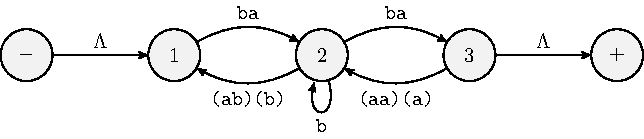
\includegraphics[]{figures/answer/Answer1A2.pdf}
                \caption*{Step 2: Bypass states 4 and 5.}
            \end{figure}
            \item Remove / bypass state 2.
            \begin{figure}[H]
                \centering
                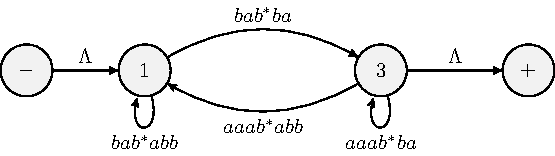
\includegraphics[]{figures/answer/Answer1A3.pdf}
                \caption*{Step 3: Bypass state 2.}
            \end{figure}
            \item Remove / bypass state 3.
            \begin{figure}[h!]
                \centering
                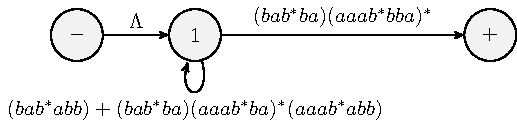
\includegraphics[]{figures/answer/Answer1A4.pdf}
                \caption*{Step 4: Removing state 3.}
            \end{figure}
            \item Remove / bypass state 1.
            \begin{figure}[h!]
                \centering
                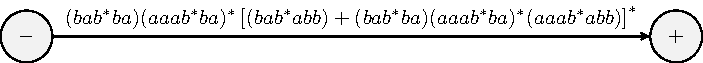
\includegraphics[]{figures/answer/Answer1A5.pdf}
                \caption*{Step 5: Removing state 1, completed regular expression.}
            \end{figure}
        \end{enumerate}
        \newpage
        \item \begin{enumerate}[label=\arabic*]
            \item 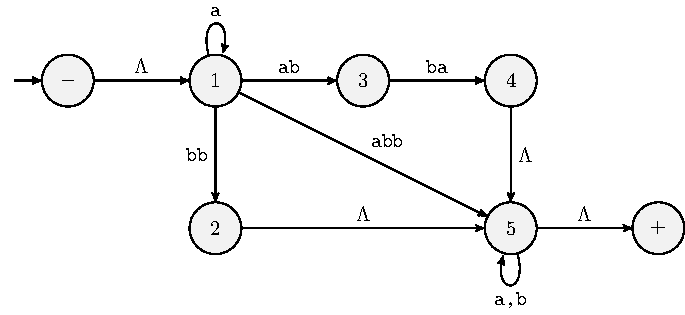
\includegraphics[]{figures/answer/Answer1B1.pdf}
            \item 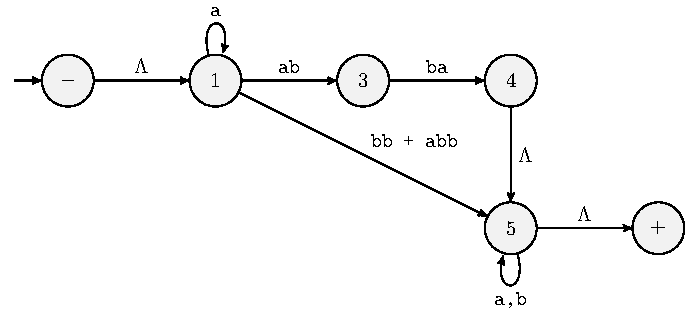
\includegraphics[]{figures/answer/Answer1B2.pdf}
            \item 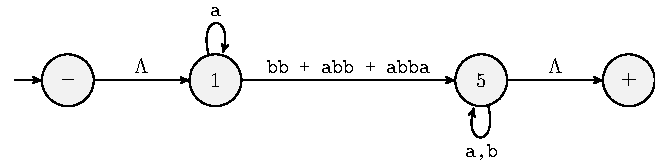
\includegraphics[]{figures/answer/Answer1B3.pdf}
            \item 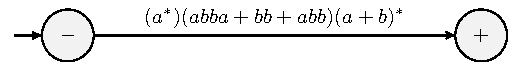
\includegraphics[]{figures/answer/Answer1B4.pdf}
        \end{enumerate}
    \end{enumerate}
\end{solution}

\begin{problem}{\#2 (110 points)}
    \begin{enumerate}[label={\bf \alph*)}]
        \item Given a TG, called \(TG1\), that accepts the language \(L1\) and a TG called \(TG2\) that accepts the language \(L2\), show how to build a new TG (called \(TG3\)) that accepts exactly the langugae \(L1L2\).
        \item Let the language \(L\) be accepted by the transition graph \(T\) and let \(L\) not contain the word \(\Lambda\).
        Show how to build a new TG that accepts all the words in \(L\) and the word \(\Lambda\).
    \end{enumerate}
\end{problem}
\vspace{2em}
\begin{solution}
    \begin{enumerate}[label=\alph*)]
        \item In order to create a new TG that accepts \(L1L2\) you would need to create a \(z\) state for every non final state in \(TG1\) reached before hitting a final state in \(TG1\).
        Once reaching a final state of \(TG1\), determine if you are continuing in \(TG1\) or moving to \(TG2\).
        \item If a TG does not accept \(\Lambda\) the start state and the final state need to be connected with a path that has no words.
        So you could either create a new edge from the start state to the end state with lambda, or make the start state also be the final state.
        This way the empty string will be accepted.
    \end{enumerate}
\end{solution}

\begin{problem}{\#3 (16 points)}
    Consider FA (1) and FA (2) at the end of this question.
    Let \(L1\) be the language accepted by FA (1) and let \(L2\) be the language accepted by FA (2).
    \begin{enumerate}[label={\bf \alph*)}]
        \item Using the algorithm of Kleene's theorem, Lemma 3, Rule 2, construct an FA for the union language \(L1 + L2\).
        \item Give an example of a word in the language \(L1 + L2\) that is also in both languages \(L1\) and \(L2\).
        \item Give a word in the language \(L1+L2\) that is in \(L1\) but not in \(L2\).
        \item Give a word in the language \(L1+L2\) that is in \(L2\) but not in \(L1\).
    \end{enumerate}
    
\end{problem}
\begin{figure}[h!]
    \hfill
    \subfigure[FA (1)]{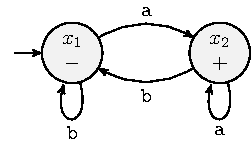
\includegraphics[width=5cm]{figures/question/Question3FA1.pdf}}
    \hfill
    \subfigure[FA (2)]{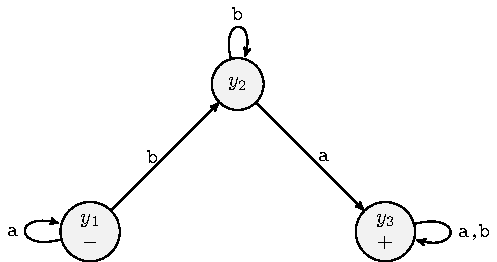
\includegraphics[width=9cm]{figures/question/Question3FA2.pdf}}
    \hfill
\end{figure}
\vspace{2em}
\begin{solution}
    \begin{enumerate}[label={\bf \alph*)}]
        \item 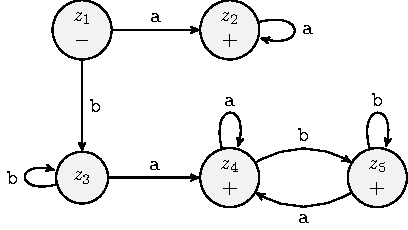
\includegraphics[]{figures/answer/Answer3A.pdf}
        \item The word \(ba\) is a member of both \(L1\) and \(L2\).
        \item The word \(a\) is a member of \(L1+L2\) and \(L1\) but not \(L2\).
        \item The word \(bab\) is a member of \(L1+L2\) and  \(L2\) but not \(L1\).
    \end{enumerate}
\end{solution}

\begin{problem}{\#4 (14 points)}
    Consider FA (2) of Q3 that accepts language \(L2\).
    \begin{enumerate}[label={\bf \alph*)}]
        \item Using the algorithm of Kleene's theorem, Lemma 3, Rule 3, construct an FA for the product language \(L2L2\).
        \item Describe (in English phrases) the language \(L2L2\) (the language accepted by part (a)).
        \item Give an example of a word with at least 5 letters that is not in the language \(L2L2\).
    \end{enumerate}
\end{problem}
\vspace{2em}
\begin{solution}
    \begin{enumerate}[label={\bf \alph*)}]
        \item 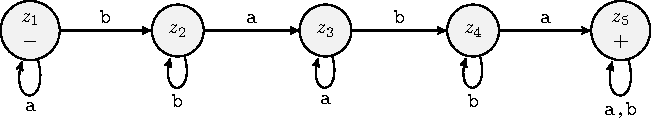
\includegraphics[]{figures/answer/Answer4A.pdf}
        \item The description of the language \(L2L2\) is alternating sets of letters.
        could have \(aabbaabb\) with any numbers of letters after.
        \item A word with 5 letters not in \(L2L2\) is \(baabb\).
        If there is an \(a\) after this word it will be accepted.
    \end{enumerate}
\end{solution}

\begin{problem}{\#5 (15 points)}
    Consider FA (1) that accepts language \(L1\) from Question 3.
    \begin{enumerate}[label={\bf \alph*)}]
        \item Using the algorithm of Kleene's theorem, Lemma 3, Rule 4, construct an FA for the language \(L1^*\).
        \item Is the language \(L1\) the same as the language \(L1^*\)?
        If so justify your answer with a brief explanation.
        If not, give an example of a word the is in one language but not the other.
    \end{enumerate}
\end{problem}
\vspace{2em}
\begin{solution}
    \begin{enumerate}[label={\bf \alph*)}]
        \item 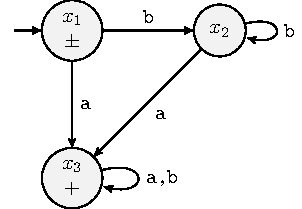
\includegraphics[]{figures/answer/Answer5A.pdf}
        \item No the language \(L1\) and \(L1^*\) are not the same language, namely the empty string \(\Lambda\) is present in \(L1^*\) but not in \(L1\).
    \end{enumerate}
\end{solution}

\begin{problem}{\#6 (14 points)}
    Consider the following Mealy machine \(\Sigma = \{a,b\}\) and \(\Gamma = \{0,1\}\).
    \begin{enumerate}[label={\bf \alph*)}]
        \item Convert this Mealy machine into a Moore machine.
        \item For input \(bbaa\), what is the output of the original Mealy machine?
        \item For input \(bbaa\) what is the output of your Moor machine?
    \end{enumerate}
\end{problem}
\begin{center}
    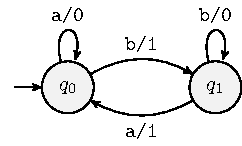
\includegraphics[width=5cm]{figures/question/Question6.pdf}
\end{center}
\vspace{2em}
\begin{solution}
    \begin{enumerate}[label={\bf \alph*)}]
        \item 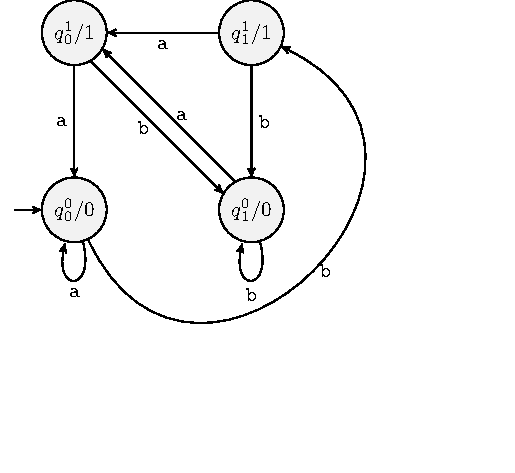
\includegraphics[]{figures/answer/Answer6A.pdf}
        \item The original mealy machine outputs \(1010\).
        \item The moore machine outputs \(1010\).
    \end{enumerate}
\end{solution}